\documentclass[10pt]{beamer}
\usetheme[
%%% option passed to the outer theme
%    progressstyle=fixedCircCnt,   % fixedCircCnt, movingCircCnt (moving is deault)
  ]{Feather}
  
% If you want to change the colors of the various elements in the theme, edit and uncomment the following lines

% Change the bar colors:
%\setbeamercolor{Feather}{bg=green!40!black}

% Change the color of the structural elements:
%\setbeamercolor{structure}{fg=green!50!black}

% Change the frame title text color:
%\setbeamercolor{frametitle}{fg=white}

% Change the normal text color background:
%\setbeamercolor{normal text}{fg=green!30!black,bg=gray!80}

% Change the block colors
%\setbeamercolor{block title}{use=structure,fg=structure.fg,bg=structure.fg!20!bg}
\setbeamercolor{block title}{use=structure,fg=white,bg=structure.fg!50!bg}
%\setbeamercolor{block body}{parent=normal text,use=block title,bg=block title.bg!50!bg}
\setbeamercolor{block body}{parent=normal text,use=block title,bg=white}

%-------------------------------------------------------
% INCLUDE PACKAGES
%-------------------------------------------------------

\usepackage[utf8]{inputenc}
%\usepackage{minted}
\usepackage[english]{babel}
\usepackage[T1]{fontenc}
\usepackage{helvet}
\usepackage{tabularx}
\usepackage{colortbl}
\usepackage{listings}

%-------------------------------------------------------
% DEFFINING AND REDEFINING COMMANDS
%-------------------------------------------------------

% colored hyperlinks
\newcommand{\chref}[2]{
  \href{#1}{{\usebeamercolor[bg]{Feather}#2}}
}

%-------------------------------------------------------
% INFORMATION IN THE TITLE PAGE
%-------------------------------------------------------

\title[Programming Merit Badge]{ }
\author{Joshua Talbot P.E.}
\institute{}
\date{28 November 2021}

%-------------------------------------------------------
% THE BODY OF THE PRESENTATION
%-------------------------------------------------------

\begin{document}

%-------------------------------------------------------
% THE TITLEPAGE
%-------------------------------------------------------

\section{Introduction}

{\1% % this is the name of the PDF file for the background


\begin{frame}{Basic Programming Concepts}{ }
\begin{center}
\begin{block}{}
\center \textbf{Welcome!}
\end{block}
\vspace{0.5cm}
\begin{figure}%%Inicia paquete para cargar figura
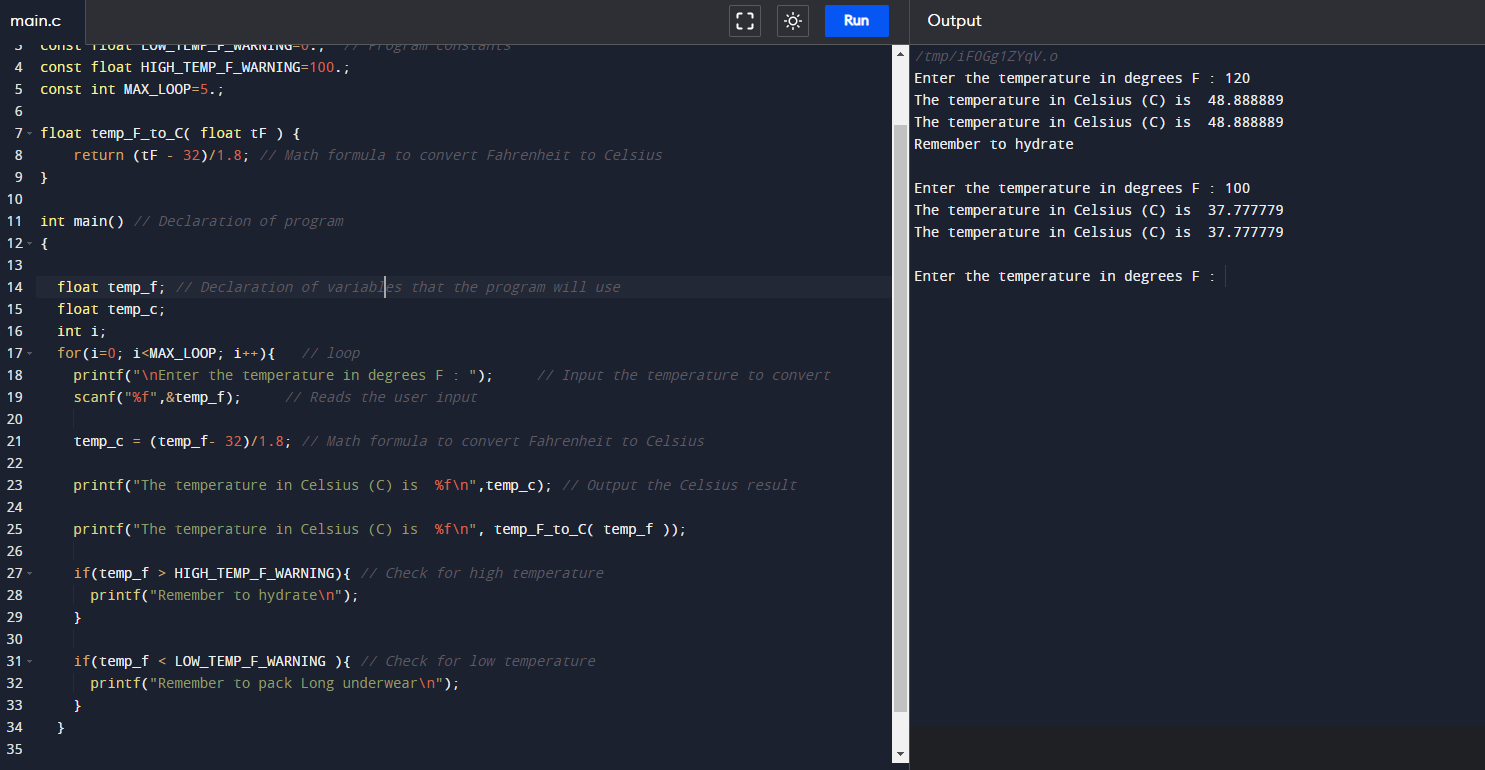
\includegraphics[width=\textwidth]{img/C_code.png}
%\caption{\label{fig:1}Programming}
\end{figure}
\end{center}
\end{frame}

%-------------------------------------------------------
% Programming History?
%-------------------------------------------------------

\begin{frame}{Who has programmed?}{ }  
\begin{block}{}
  \begin{itemize}
    \item {\tt What languages have you tried to program in?}
    \item {\tt Do you have a favorite?  Why?}
    \item {\tt Do you know how to type?}
    \item {\tt What computer experience do you have?}
    \end{itemize}
  \end{block}
\end{frame}

%-------------------------------------------------------
% Lets Get Started...
%-------------------------------------------------------

\begin{frame}{Starting a Program}{ }  
\begin{block}{}
  \begin{itemize}
    \item {The best programmers don't start by coding.}
    \item {The best programmers plan first.  They write the requirements and generate diagrams to help plan out the code they write.}
    \item {Then they use this to generate pseudo code.}
    \item {Then the actual programming begins.}
    \end{itemize}
  \end{block}
\end{frame}

%-------------------------------------------------------
% pseudo code...
%-------------------------------------------------------

\definecolor{backcolour}{rgb}{0.95,0.95,0.92}
\definecolor{codegreen}{rgb}{0,0.6,0}

% Define a custom style
%\lstdefinestyle{myStyle}{
%    backgroundcolor=\color{backcolour},   
%    commentstyle=\color{codegreen},
%    basicstyle=\footnotesize,
%    breakatwhitespace=false,         
%    breaklines=true,                 
%    keepspaces=true,                 
%    numbers=left,       
%    numbersep=5pt,                  
%    showspaces=false,                
%    showstringspaces=false,
%    showtabs=false,                  
%    tabsize=2,
%}

\lstdefinestyle{myStyle1}{
    belowcaptionskip=1\baselineskip,
    breaklines=true,
    frame=none,
    numbers=left,
    numbersep=5pt,
    showspaces=false,                
    showstringspaces=false,
    showtabs=false,                  
    tabsize=2,
    basicstyle=\scriptsize,
    keywordstyle=\bfseries\color{green!40!black},
    commentstyle=\color{purple!40!black},
    identifierstyle=\color{blue},
    backgroundcolor=\color{gray!10!white},
    tabsize=4,
}

\lstdefinestyle{myStyle_LF}{
    belowcaptionskip=1\baselineskip,
    breaklines=true,
    frame=none,
    numbers=left,
    numbersep=5pt,
    showspaces=false,                
    showstringspaces=false,
    showtabs=false,
    basicstyle=\small,
    keywordstyle=\bfseries\color{green!40!black},
    commentstyle=\color{purple!40!black},
    identifierstyle=\color{blue},
    backgroundcolor=\color{gray!10!white},
    tabsize=4,
}

\lstset{style=myStyle_LF}

\begin{frame}[fragile]{Pseudo Code}{ }
\lstinputlisting[caption=Sample Code Listing Python, label={lst:listing-python}, language=Python,firstline=1,lastline=15]{code/calc_adder_pseudo.py}
\end{frame}

%-------------------------------------------------------
% Variables
%-------------------------------------------------------

}
{\3% % this is the name of the PDF file for the background

\begin{frame}{Variables}{}
\begin{block}{}
Variables are the backbone of all programming languages.  They are used to store important information for the programmer.  The programmer can then use this stored information at a later point in the program.\end{block}
\begin{block}{Examples}
\begin{itemize}
    \item We store names in memory to recall them later to obtain that person's attention.
    \item When hiking we store the path color or the the next direction we need to head in memory so when we see the next marker or trail we can make a decision of the direction to head.
\end{itemize}
\end{block}
\end{frame}

%-------------------------------------------------------
% Control Structures
%-------------------------------------------------------

\begin{frame}{Control Structures}{}
\begin{block}{Decision Making (conditionals)}
\begin{itemize}
    \item \textbf{If, If/Else}: Used to compare variables aganist a value or another variable to make a decision.
    \item \textbf{Case/Switch}: Similar to several stacked single if tests.
\end{itemize}

\end{block}
\begin{block}{Loops (iteration)}
    \begin{itemize}
    \item \textbf{While loops} execute and continue to execute repeated time at the onset and verification of a logical condition. The condition is tested at the start of every loop iteration.
    \item \textbf{For loops} execute for a prescribed number of times, as controlled by a counter or an index.
    \end{itemize}
\end{block}
\end{frame}

%-------------------------------------------------------
% Implementation - Program Development
%-------------------------------------------------------

\begin{frame}[fragile]{Pseudo Code}{ }
\begin{block}{}
\lstset{style=myStyle_LF} 
\lstinputlisting[caption=Sample Code Listing Python, label={lst:listing-python}, language=Python,firstline=1,lastline=15]{code/calc_adder_pseudo.py}
\end{block}
\end{frame}

\begin{frame}[fragile]{File Header}{ }
\begin{block}{}
\lstset{style=myStyle_LF} 
\lstinputlisting[caption=Sample Code Listing Python, label={lst:listing-python}, language=Python,firstline=1,lastline=9]{code/calc_adder_pseudo.py}
\end{block}
\end{frame}

\begin{frame}[fragile]{Pseudo Code}{ }
\begin{block}{}
\lstset{style=myStyle_LF}  
\lstinputlisting[caption=Sample Code Listing Python, label={lst:listing-python}, language=Python,firstline=10,lastline=15]{code/calc_adder_pseudo.py}
\end{block}
\end{frame}

}

{\4 % % this is the name of the PDF file for the background

\begin{frame}[fragile]{LETS CODE: Implement User Input...}{ }  
\begin{block}{}
\lstset{style=myStyle_LF}
\lstinputlisting[caption=Sample Code Listing Python, label={lst:listing-python}, language=Python,firstline=12,lastline=18]{code/calc_adder_input.py}
\end{block}
\end{frame}

\begin{frame}[fragile]{LETS CODE: Perform the Math.}{ }
\begin{block}{}
\lstset{style=myStyle_LF}
\lstinputlisting[caption=Sample Code Listing Python, label={lst:listing-python}, language=Python,firstline=17,lastline=21]{code/calc_adder.py}
\end{block}
\end{frame}

\begin{frame}[fragile]{Addition Calculator}{ }
\begin{block}{}
\lstset{style=myStyle1}
\lstinputlisting[label={lst:listing-python}, language=Python]{code/calc_adder.py}
\end{block}
\end{frame}

\begin{frame}
  \begin{block}{}
  {\huge Good Luck with the Programming!}
  \end{block}
\end{frame}}
\end{document}
}